\chapter{CipherText Policy Attribute Based Encryption}

% \section{Literature Review}


In ciphertext-policy attribute-based encryption (CP-ABE) ,a user's private key will be associated with an arbitrary number of attributes expressed as strings,from the universe of attributes available. 
On the other hand, when a party encrypts a message in our system, they specify an associated access structure over attributes. A user will only be able to decrypt a ciphertext if that user’s attributes pass through the ciphertext’s access structure. 


   At a mathematical level, access structures in our system are described by a monotonic “access tree”, where nodes of the access structure are composed of threshold gates and the leaves describe attributes. We note that AND gates can be constructed as n-of-n threshold gates and OR gates as 1-of-n threshold gates. Furthermore, we have implemented more complex access controls such as numeric ranges by converting them to smaller access trees using 0-1 Encoding for comparison.
\begin{figure}
    \centering
    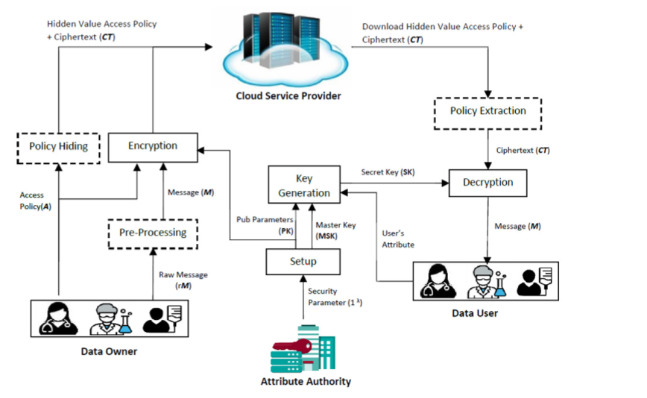
\includegraphics[width=0.8\linewidth]{Images/CBCArchitecture.jpeg}
    \caption{Standard Archicture of CP-ABE}
    \label{fig:enter-label}
\end{figure}
    A ciphertext-policy attribute based encryption scheme consists of four fundamental algorithms: Setup, Encrypt, KeyGen, and Decrypt. In addition, we allow for the option of a fifth algorithm Delegate.

    \begin{enumerate}
    \item Setup\par
 The setup algorithm takes no input other than the implicit security parameter. It outputs the public parameters PK and a master key MK.
    \item Encrypt(PK,M, A)\par
   The encryption algorithm takes as input the public parameters PK, a message M, and an access structure A over the universe of attributes. The algorithm will encrypt M and produce a ciphertext CT such that only a user that possesses a set of attributes that satisfies the access structure will be able to decrypt the message. We will assume that the ciphertext implicitly contains A.
    \item Key Generation(MK,S)\par
   The key generation algorithm takes as input the master key MK and a set of attributes S that describe the key. It outputs a private key SK.
    \item Encrypt(PK,M, A) \par
   The encryption algorithm takes as input the public parameters PK, a message M, and an access structure A over the universe of attributes. The algorithm will encrypt M and produce a ciphertext CT such that only a user that possesses a set of attributes that satisfies the access structure will be able to decrypt the message. We will assume that the ciphertext implicitly contains A.
    \item Decrypt(PK, CT, SK) \par
  The decryption algorithm takes as input the public parameters PK, a ciphertext CT, which contains an access policy A, and a private key SK, which is a private key for a set S of attributes. If the set S of attributes satisfies the access structure A then the algorithm will decrypt the ciphertext and return a message M.
  \item Delegate(SK, S ̃) \par
 The delegate algorithm takes as input a secret key SK for some set of attributes S and a set S ̃⊆ S. It output a secret key SK for the set of  ̃ attributes S ̃.
\end{enumerate}





